\documentclass{mprop}
\usepackage{graphicx}

% alternative font if you prefer
%\usepackage{times}

% for alternative page numbering use the following package
% and see documentation for commands
%\usepackage{fancyheadings}


% other potentially useful packages
%\uspackage{amssymb,amsmath}
%\usepackage{url}
%\usepackage{fancyvrb}
%\usepackage[final]{pdfpages}

\begin{document}

%%%%%%%%%%%%%%%%%%%%%%%%%%%%%%%%%%%%%%%%%%%%%%%%%%%%%%%%%%%%%%%%%%%
\title{Model Reuse Paradigm in Edge Computing}
\author{Xenia Skotti}
\date{Decemeber 2021}
\maketitle
%%%%%%%%%%%%%%%%%%%%%%%%%%%%%%%%%%%%%%%%%%%%%%%%%%%%%%%%%%%%%%%%%%%

%%%%%%%%%%%%%%%%%%%%%%%%%%%%%%%%%%%%%%%%%%%%%%%%%%%%%%%%%%%%%%%%%%%
\tableofcontents
\newpage
%%%%%%%%%%%%%%%%%%%%%%%%%%%%%%%%%%%%%%%%%%%%%%%%%%%%%%%%%%%%%%%%%%%

%%%%%%%%%%%%%%%%%%%%%%%%%%%%%%%%%%%%%%%%%%%%%%%%%%%%%%%%%%%%%%%%%%%
\section{Introduction}\label{intro}

Lee et al. \cite{ComputeReuse} define compute reuse as "the partial or full utilization of already executed computational task results by multiple users to complete a new task while avoiding computation redundancy".  Systems that adopt compute reuse benefit from significant performance gains motivating model reuse in machine learning (ML). Model reuse \cite{Learnware} attempts to construct a model from other pre-existing and pretrained models for other tasks, in order to avoid building a model from scratch. Exploitation of pre-existing models can set a good basis for the training of a new model which translates into a reduced time cost, data amount and expertise required to train a new model. Moreover, model reuse has been used to tackle concept drift \cite{ConceptDrift} and building ad-hoc analytic models \cite{MaterializationReuse}.

Model reusability is compelling and therefore both theoretical \cite{Learnware} and empirical \cite{MaterializationReuse}\cite{KernelMMD}  frameworks have been proposed to take advantage of it. Many of the approaches proposed, involve a two-phased framework of a preprocessing and runtime phase. In the preprocessing phase, the model and its data are shared in a pool from which in the runtime phase the relevant ML models are identified. Consider the case of edge computing, where given a number of nodes and their corresponding datasets we want to decide for which nodes to train a distinct model and for which to reuse one. In this context the reuse comes from the fact that we don’t train a model for all the nodes but instead reuse one of the existing ones. A framework for model reuse in edge computing requires it is online hence, these steps are merged and to the best of our knowledge no such framework has been proposed. 

%%%%%%%%%%%%%%%%%%%%%%%%%%%%%%%%%%%%%%%%%%%%%%%%%%%%%%%%%%%%%%%%%
\section{Statement of Problem}

Our project aims to contribute a novel online framework for model reuse in edge computing, which given a set of nodes and their corresponding datasets can determine for which nodes to train distinct models and for which nodes to reuse one. Therefore, we need to be able to determine both if nodes' datasets are similar but also the direction of reusability i.e. if one node's model would be better suited than the other. Avoiding the need to train models for all of the nodes in the network reduces the amount of computational resources that would be required if no reuse was applied. Consequently, the network can benefit from overall improved performance. Additionally, compared to other model reuse frameworks which the two distinct steps to be executed at different points in time, our framework carries out both steps at a single point in time i.e. it is online. 
 
%%%%%%%%%%%%%%%%%%%%%%%%%%%%%%%%%%%%%%%%%%%%%%%%%%%%%%%%%%%%%%%%%%%
\section{Literature Survey}

Compute reuse has been investigated in the context of edge computing by \cite{ComputeReuse} to quantify its gain. Executing experiments on three applications: matrix multiplication, face detection, and chess, they found that systems that adopt compute reuse, compared to systems that don't, can finish the same task up to five times faster. In addition to the benefits of compute reuse they also highlight some challenges including task representation and privacy considerations. Model tasks need to have a clear specification detailing their purpose and speciality in order to identify when they can be re-used while also preserving user privacy when they are shared. Motivated by similar concerns a theoretical paradigm named learnware was proposed by Zhou \cite{Learnware}. More specifically, a learnware is a machine learning model that is pretrained and achieves good performance paired with a detailed specification. The vision behind the paradigm was that learnware models can be shared in a pool without their raw data, allowing data scientists to identify pretrained models that satisfy their requirements without concerns over privacy violations. Therefore, the author identified three characteristics: reusable, evolvable and comprehensible as fundamental for a model to be considered a learnware.  

Based on this paradigm, the reduced kernel mean embedding (RKME) \cite{KernelMMD} was presented, a two phased framework consisting of the upload and deployment phase. During the upload phase, each model is paired with its kernel mean embedding (KME) of the dataset and added to the pool of models. Roughly speaking, a kernel mean embedding is a point in the reproducing Hilbert space (RKHS) which "summarises" the probability distribution. Then in the deployment phase either a single or a combination of models is chosen based on the RKHS distance between the testing (target) mean embedding and reduced (source) embedding of pool models. Therefore, there is no need to access the raw data since KME acts a proxy for them. The RKME method is similar to the MMD  statistic \cite{OriginalMMD}, which is the largest difference between the mean embedding of two populations (source and target) and its aim is to determine if the two populations were drawn from the same distribution. Essentially, this is what the deployment phase of the framework does, it wants to find the model which minimises the difference and thus ensures that the target distribution is the same as the source. The framework was tested in a series of experiments including a real-world project where it outperformed reuse baselines in terms of the root-mean-square error.

The author of the learnware paradigm \cite{Learnware} recognises transfer learning as a preliminary attempt to reusability. The aim of transfer learning is to transfer the knowledge of a pretrained model to a new model that is used for a different but related problem. In transfer learning there are three key research issues as identified in \cite{DefinitionTL}: when, how and what to transfer. This corresponds to identifying a source domain that would benefit the target domain, then using an algorithm the transferable knowledge across domains is discovered. A two-stage framework dubbed as Learning to Transfer (L2T) was presented \cite{L2T}, which exploits previous transfer learning experiences to optimize what and how to transfer between domains. In the first stage each transfer learning experience is encoded into three parts: a pair of source and target domains, the transferred knowledge between them represented by latent factors and the performance improvement ratio. Using these transfer learning experiences, L2T learns a reflection function, which approximates the performance improvement ratio and thus encrypts transfer learning skills of deciding what and how to transfer. The improvement ratio in this framework is the difference between domains calculated by MMD further highlighting the similarity to RKME \cite{KernelMMD}. In addition to the MMD between domains, the variance is also calculated since a small MMD paired with an extremely high variance still indicates little overlap. A potential drawback of the RKME \cite{KernelMMD} framework, and by extension the learnware paradigm, is that the variance between pairs cannot be calculated since the raw data are not available during the testing phase. During the second stage, whenever a new pair of domains arrives, L2T optimizes the knowledge to be transferred by maximising the value of the learned reflection function.

Concerns over intellectual property (IP) infringement and vulnerability propagation of deep learning models (DNN) motivated the proposal of ModelDiff \cite{DNNSimilarity}, a testing-based approach to DNN model similarity comparison. They compare the decision logic of models on the test inputs represented by a decision distance vector (DDV),a newly defined data structure in which each value is the distance between the outputs of the model produced by two inputs. These inputs are pairs of normal and corresponding adversarial samples and thus when used to calculate the DDV, the decision boundary is captured. In contrast to RKME \cite{KernelMMD} which is a compute reuse framework, ModelDiff is a model reuse detector. 

Model reuse has also been used to handle concept drift, a situation where the distribution of the data (usually stream data) changes. The assumption that previous data contain some useful information, indicates that the models corresponding to the data can be leveraged. Condor was proposed \cite{ConceptDrift} as an approach to handling concept drift through model reuse. Condor consists of two modules, ModelUpdate and WeightUpdate which leverage previous knowledge to build new model, hence updating the model pool and adapt the weights of previous models to reflect current reusability performance respectively. The effectiveness of the approach was validated using both synthetic and real-world datasets. 

Hasani et al. \cite{MaterializationReuse} proposed a two-phased approach, to build faster models for a popular class of analytic queries by leveraging model reuse. Similar to other approaches such as RKME \cite{KernelMMD}, there is a preprocessing and a runtime phase. During the first phase the models, their statistics and some meta-data are stored, while in the second phase relevant models are identified from which an approximate model is constructed. Moreover, they propose two methods for generating approximate models, one which is extremely fast but does not provide a fine-tuning option and another which does at the cost of efficiency. Their approach can achieve speed-ups of several orders on magnitude on very large datasets, however it is only geared towards exploratory analysis purposes and the approach is potentially less robust under concept drift. 

Lee et al. \cite{ComputeReuse} also discuss alternative approaches and corresponding challenges of compute reuse including in networks. They identify that reuse can be achieved either in a distributed or centralized manner. The distributed approach involves forwarding tasks to the compute reuse node that is responsible for the operation. This adds additional complexity to the forwarding operations of routers resulting in a potential downgrade in performance. Reuse of results in a network setting undoubtedly improves performance, however speeding up the estimation of parameters can also be beneficial in that regard. Nodes in a network can collaborate to estimate parameters as discussed in \cite{DistributedEstimation}. More specifically, their method takes advantage of the joint sparsity of vectors used for computations enhancing estimation performance. Joint sparsity simply means that the indexes of nonzero entries for all nodes are the same, but their values differ.  The authors also adopt an intertask cooperation strategy to consider intertask similarities. Their method assumes that both the vectors of interest and their associated noise follow a zero-mean Gaussian distribution which is a strong assumption for the data to hold.

In conclusion, reusing models results in significant reduction in compute usage resources. Both theoretical and empirical frameworks have been proposed to take advantage of the performance improvement of model reusability. Nevertheless, model reuse has also been used to tackle concept drift and building ad-hoc analytic models. While model reuse is undoubtedly beneficial many have raised concerns including user privacy and intellectual property considerations. These are legitimate concerns of model sharing, however  our model reuse  framework is novel and therefore user privacy is not a concern at this stage of development. In the future we could amend the framework to not expose any data outside of the node. At this stage we're interested in whether the framework is feasible. In contrast to previous research in which frameworks required two distinct steps, our framework is online, and they are therefore merged. Our framework includes determining which datasets are similar, but also the direction of reusability.  Similarly, to the L2T \cite{L2T} framework we use MMD to measure the similarity of two dataset domains. In previous research there was no requirement to determine the direction of reusability hence we propose a novel approach, using an One-class Support Vector Machine (OCSVM)  model of each node to predict other node’s inliers and measuring the overlap.

%%%%%%%%%%%%%%%%%%%%%%%%%%%%%%%%%%%%%%%%%%%%%%%%%%%%%%%%%%%%%%%%%%%
\section{Proposed Approach}

% Show that your proposed approach is feasible, but identify any risks. Give a report on your progress thus far, describing the state of your feasibility study, proof of concept, or prototype that demonstrate you are capable of completing your project.

In this section we elaborate on the implementation of our proposed approach and the corresponding a experimental setup to test out our framework along with a summary of the results of the experiments executed so far.

\subsection{Detailed Framework Implementation}

\begin{algorithm}
    \DontPrintSemicolon
    \caption{Calculates the average similarity MMD (ASMMD) between the given nodes.
    }\label{alg:asmmd}
    
    \KwData{$\boldsymbol{samples}$: dictionary associating each node (pi2-pi5) with a sample used for the MMD calculation, $\boldsymbol{similar\_nodes}$: nodes which we have visually identified as similar to each other, $\boldsymbol{other\_nodes}$: the rest of the nodes, $\boldsymbol{kernel}, \boldsymbol{bandwidth}$: the kernel type and scalar value to be used for the MMD calculation.}
    \KwResult{ASMMD}

    \Begin{ 
        \tcp{Calculating the baseline ASMMD}
        $similar\_mmds \longleftarrow \left[\right]$ \;
        \SetAlgoLined
        \SetKw{KwTo}{in}
        \For{$x, y$ \KwTo $get\_pair\_combos(similar\_nodes)$}{
            $sx \longleftarrow samples[x]$, $sy \longleftarrow samples[y]$ \;
            $mmd \longleftarrow MMD(sx, sy, kernel, bandwidth)$ \;
            $similar\_mmds.append(mmd)$ \;
        }
        \tcp{Compare whether any of the other\_nodes are similar to any of the similar\_nodes using the baseline ASMMD}
        \For{$x$ \KwTo $other\_nodes$}{
            $sx \longleftarrow samples[x]$ \;
            \For{$y$ \KwTo $similar\_nodes$}{
                $sy \longleftarrow samples[y]$ \;
                $mmd \longleftarrow MMD(sx, sy, kernel, bandwidth)$ \;
                $current\_asmmd \longleftarrow \boldsymbol{mean}(similar\_mmds)$ \;
                \If{$mmd < (current\_asmmd + 1) * 0.05$}{
                    $similar\_mmds.append(mmd)$}
            }
        }
        \tcp{Compare whether any of the other\_nodes are similar to each other using the current ASMMD}
        \If{$\boldsymbol{len}(other\_nodes>1)$}{
            \For{$x, y$ \KwTo $get\_pair\_combos(other\_nodes)$}{
                $sx \longleftarrow samples[x]$, $sy \longleftarrow samples[y]$ \;
                $mmd \longleftarrow MMD(sx, sy, kernel, bandwidth)$ \;
                $current\_asmmd \longleftarrow \boldsymbol{mean}(similar\_mmds)$ \;
                \If{$mmd < (current\_asmmd + 1) * 0.05$}{
                    $similar\_mmds.append(mmd)$}
            }
        }
        $asmmd = \boldsymbol{mean}(similar\_mmds)$ \;
    }
\end{algorithm}

Our online model reuse framework needs to be able to determine two things given a pair of nodes. First and foremost, one of the fundamental requirements of any model reuse framework is to be able to choose the model that best fits the (test) data of the target domain. One of the ways this can be achieved is by finding the model whose source domain (training data) is drawn from the same distribution as the target domain. Therefore, the difference between domains needs to be quantified and minimised to find the best model. This is essentially what the Maximum Mean Discrepancy (MMD) \cite{OriginalMMD} statistic does. In addition to measuring the similarity between two dataset domains, we need to determine the direction of reusability. In other frameworks where the reused model originated from a pool there was no such requirement because there was only one direction of reusability, the pool. In this setting though there are two directions per pair, and we need to define a method to do so. A simple solution to this, is to measure the overlap between the inlier points of two datasets. Any dataset is expected to have a few outliers and a simple filtering technique would be to use One-class Support Vector Machines (OCSVM) \cite{OriginalOCSVM} to determine which points are inliers.  The method, first presented by Schölkopf et. al \cite{OriginalOCSVM},  utilizes a training data set with normal data to learn the boundaries of the normal data points. Therefore, data points which lie outside of the region to be classified as outliers. Given two nodes and their corresponding OCSVM models, we can use each OCSVM model to predict the other node's inliers and then find the probability of detecting them, hence their overlap. 

Initially, we were investigating whether either MMD or OCSVM or both could be used to detect similar pairs.  Upon some initial analysis, the OCSVM method was not stable but nevertheless the probability of detecting inliers was still a useful piece of information to determine direction of reusability. Hence, we've adapted our method to using MMD to detect similar pairs and OCSVM the direction of reusability. 

Using the MMD two samples are drawn from the same distribution if it is zero. However, we're using an estimate and thus in this case, we need to set a threshold for what score would be deemed similar. We've dubbed this threshold to be the average similarity MMD (ASMMD) and we've devised an algorithm to allow us to calculate it (Algorithm \ref{alg:asmmd}). The algorithm requires that we categorise nodes into two sets, one where all nodes are similar to each other and the rest of them. We calculate a baseline ASMMD by calculating the MMD of all pair combinations of the similar nodes. Then, we use ASMMD (allowing for a 5\% variation) to judge whether the rest of the nodes are similar to each other or to the similar nodes. If they are we calculate the new ASMMD and we use this to judge the next pair. Using the result of this process we can then judge which pairs are similar for a given experiment. After we've identified the similar pairs we find the direction of reusability using their OCSVM models. We can use one node's model to predict the other node's inliers and then find the probability of detecting them. 

\subsection{Experimental Setup}

\subsubsection{Training Data}

In order to test the feasibility of our framework we first need a dataset. For the purposes of our framework we've experimented with the \textbf{\textit{GNFUV Unmanned Surface Vehicles Sensor Data Set}} \cite{Dataset} which includes data from three experiments. In each experiment there are four sets of mobile sensor readings data recorded by the Raspberry Pi's corresponding to four Unmanned Surface Vehicles (USVs). Each node (USV) dataset contains the humidity and temperature recorded when they were floating over the sea surface in a GPS pre-defined trajectory in a coastal area of Athens (Greece). The data description and visualisation can be found in Table \ref{tab:Data Description} and Figure \ref{fig:Data Visualisation} respectively.

\begin{figure}
% \centering
    \begin{subfigure}{0.5\textwidth}
      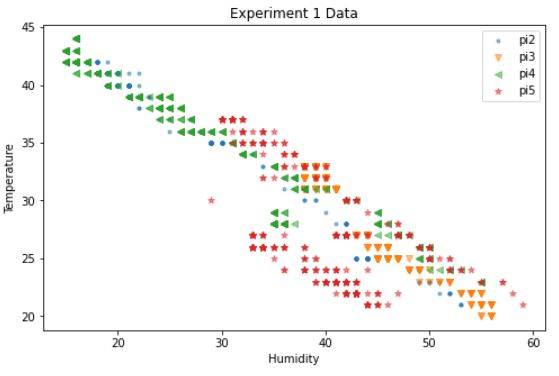
\includegraphics[width=1\linewidth]{mprop/exp1.JPG}
      \label{fig:sfig2}
    \end{subfigure}
    \begin{subfigure}{0.5\textwidth}
      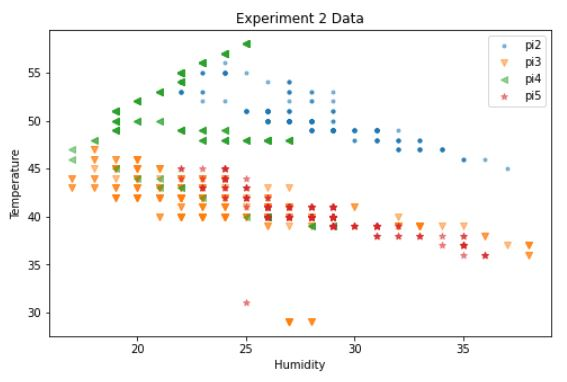
\includegraphics[width=1\linewidth]{mprop/exp2.JPG}
      \label{fig:sfig2}
    \end{subfigure}
\end{figure}

\setcounter{figure}{0}
\begin{figure}
    \centering
    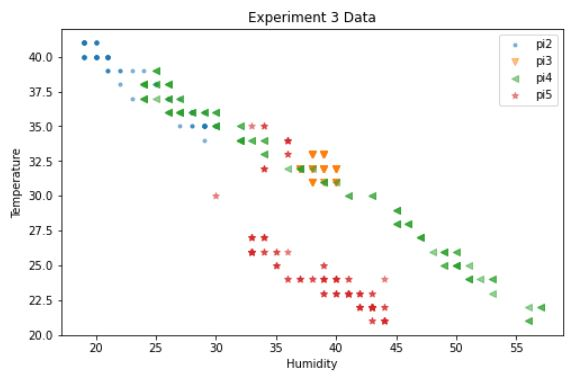
\includegraphics[width=0.5\linewidth]{mprop/exp3.JPG}
    \caption{Data visualisation per experiment}
    \label{fig:Data Visualisation}
\end{figure}

\begin{table}[]
\centering
\begin{tabular}{|cccccccccc|}
\hline
\multicolumn{10}{|c|}{\textbf{Experiment 1}}                                                                                                                                   \\ \hline
\multicolumn{1}{|c|}{\textbf{Node}} & \multicolumn{1}{c|}{\textbf{No. of Entries}} & \multicolumn{4}{c|}{\textbf{Humidity}}        & \multicolumn{4}{c|}{\textbf{Temperature}} \\ \hline
\multicolumn{1}{|c|}{\textbf{}}     & \multicolumn{1}{c|}{\textbf{}}               & Min & Max & Avg   & \multicolumn{1}{c|}{Std}  & Min     & Max     & Avg       & Std       \\
\multicolumn{1}{|c|}{pi2}           & \multicolumn{1}{c|}{1532}                    & 3   & 45  & 35.85 & \multicolumn{1}{c|}{6.57} & 15      & 57      & 27.6      & 11.08     \\
\multicolumn{1}{|c|}{pi3}           & \multicolumn{1}{c|}{899}                     & 19  & 33  & 28.53 & \multicolumn{1}{c|}{4.39} & 34      & 59      & 43.04     & 6.17      \\
\multicolumn{1}{|c|}{pi4}           & \multicolumn{1}{c|}{1766}                    & 18  & 45  & 35.47 & \multicolumn{1}{c|}{6.55} & 0       & 64      & 28.2      & 11.71     \\
\multicolumn{1}{|c|}{pi5}           & \multicolumn{1}{c|}{2078}                    & 18  & 37  & 27.51 & \multicolumn{1}{c|}{5.1}  & 20      & 63      & 39.78     & 6.9       \\ \hline
\multicolumn{10}{|c|}{\textbf{Experiment 2}}                                                                                                                                   \\ \hline
\multicolumn{1}{|c|}{pi2}           & \multicolumn{1}{c|}{580}                     & 26  & 56  & 48.48 & \multicolumn{1}{c|}{6.6}  & 21      & 49      & 28.42     & 3.86      \\
\multicolumn{1}{|c|}{pi3}           & \multicolumn{1}{c|}{807}                     & 27  & 49  & 41.73 & \multicolumn{1}{c|}{4.14} & 17      & 46      & 23.41     & 5.66      \\
\multicolumn{1}{|c|}{pi4}           & \multicolumn{1}{c|}{1021}                    & 30  & 59  & 50.56 & \multicolumn{1}{c|}{6.4}  & 16      & 36      & 22.76     & 2.76      \\
\multicolumn{1}{|c|}{pi5}           & \multicolumn{1}{c|}{1407}                    & 30  & 48  & 40.13 & \multicolumn{1}{c|}{2.73} & 20      & 49      & 28.05     & 3.36      \\ \hline
\multicolumn{10}{|c|}{\textbf{Experiment 3}}                                                                                                                                   \\ \hline
\multicolumn{1}{|c|}{pi2}           & \multicolumn{1}{c|}{342}                     & 33  & 42  & 38.39 & \multicolumn{1}{c|}{2.39} & 17      & 31      & 23.44     & 4.09      \\
\multicolumn{1}{|c|}{pi3}           & \multicolumn{1}{c|}{264}                     & 27  & 33  & 31.95 & \multicolumn{1}{c|}{0.77} & 34      & 43      & 38.63     & 1.26      \\
\multicolumn{1}{|c|}{pi4}           & \multicolumn{1}{c|}{488}                     & 20  & 39  & 31.24 & \multicolumn{1}{c|}{5.31} & 23      & 59      & 38.28     & 10.56     \\
\multicolumn{1}{|c|}{pi5}           & \multicolumn{1}{c|}{555}                     & 21  & 37  & 25.23 & \multicolumn{1}{c|}{3.91} & 20      & 47      & 38.13     & 4.65      \\ \hline
\end{tabular}
\caption{\label{tab:Data Description}Dataset Description}
\end{table}

\subsubsection{Classifier of Choice}

Using the humidity and temperature attributes of the dataset we have trained regression models to capture the relationship between humidity and temperature. The classifier of choice is Support Vector Regression Machine's (SVRs). SVRs are a version of SVM for regression proposed by Vapnik et al. \cite{OriginalSVR}. The adaptation is accomplished by introducing an $\epsilon$-insensitive region around the function, called the $\epsilon$-tube as shown in Figure \ref{fig-SVRex}. Similarly to other SVM methods, the hyperplane is represented in terms of support vectors, which are training samples that lie outside the boundary of the tube.  The optimization problem objective is to find the tube that best approximates the continuous-valued function, while balancing model complexity and prediction error. Therefore, the goal is to first minimise an $\epsilon$-insensitive loss function and find the flattest tube that contains most of the training instances. Therefore, SVRs have a few variables of interest we want to optimise for each node model. It is worth nothing that we experiment with both the linear and rbf kernels in order to determine which is better suited for our framework. We optimise the regularization parameter and the epsilon in the epsilon-SVR model using grid search given a node's dataset.

\begin{figure}
\begin{center}
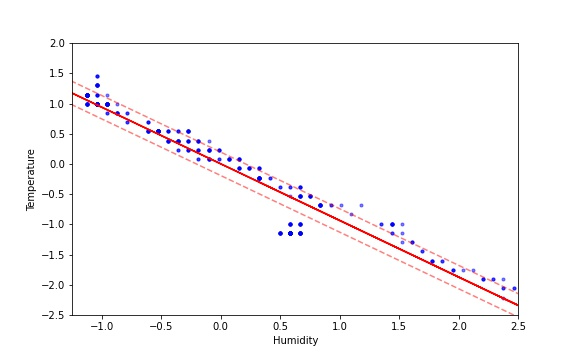
\includegraphics[scale=0.45]{SVR_representation.jpg}
\end{center}
\caption{\label{fig-SVRex}Visual Representation of an SVR}
\end{figure}

\subsubsection{Evaluation}

The aim of the project is to test whether we can detect similar pairs and the direction of reusability using MMD and OCSVM respectively. In order to test this hypothesis we need to find the similar pairs of nodes in the experiments e.g. (pi2, pi4) and which node's model to replace which  i.e. forward (pi2, pi4) or backward (pi4, pi2). Once we identify the pairs, assume that we have identified them to be (pi3, pi5) and (pi2, pi4), we will train and optimise a model for each node (using Grid Search) and then for each pair we will one node's model on their counterpart i.e. pi3 model on pi5 and the pi5 model on pi3 to determine if the given direction of reusability given by OCSVM is correct. We can test the correctness of MMD using the discrepancy error, the absolute difference between the predicted coefficient of determination (i.e. score given when using the counterpart model to make predictions) and the actual coefficient of determination (i.e. score when using the native model of the node). This can measure the drop in performance and hence whether this is a good pair for reusability. Now to test the correctness of the direction of reusability indicated by OCSVM we measure if using the node indicated by OCSVM will result in a better reusability model for both nodes instead of the other way around. 

In our experiments we wanted to investigate the feasibility of our framework while also taking into account some variables of interest that can affect results. For example, the choice of kernel for SVR impacts how over-fitted the model is and hence how it responds when it is reused. Additionally, we choose to optimise parameters for SVR models in order to get the best model for each node individually and compare with the reusability performance. Additionally, we've experimented with 3 distinct networks whose sample size varies and hence testing our framework in different contexts. Lastly, we've used both the original and standardised version of the data to investigate the effect of variance on the framework.

\subsection{Current Results}\label{section:CR}

From our initial experiments we have found the following. First, for all pairs (forward, backward) non-linear models have higher baseline scores however this does not always translate into better reusability scores. Pairs where both models have good baseline scores are good models for reusability on both sides and for this to be true data need to be standardised. When data are non-standardised OCSVM scores need to be high on both sides for this to be true. Additionally, when data are standardised for all experiments OCSVM correctly predicts the direction for reusability for the model that yields the best results the majority of the time. Granted in some cases the opposite direction can have a better model if the correct model is not chosen. However, when data are not standardised, this is only true for experiment 1 as for the rest of them it is either partially true or untrue. Therefore, OCSVM seems to be more stable when data are standardised.  We suspect this is due to minimisation of variance in the data. MMD is generally stable except in experiment 3 for non-standardised data. Therefore, we've identified the following differences across experiments. Experiments 1 \& 2 provide generally consistent results for both standardised and non-standardised data.  Experiment 3 has the most variability in results when comparing standardised to non-standardised data. It is worth mentioning that the sample sizes of experiments decrease, and this may be the issue since Experiments 1 \& 3 show similar visual characteristics.

To summarise, we've provided a detailed description of our framework implementation along with the experimental set up and the experiments executed so far.

%%%%%%%%%%%%%%%%%%%%%%%%%%%%%%%%%%%%%%%%%%%%%%%%%%%%%%%%%%%%%%%%%%%
\section{Work Plan}

% show how you plan to organize your work, identifying intermediate deliverables and dates.

Based on the issues identified in section \ref{section:CR}, we plan to increase the sample size for data originating from experiment 3 to test whether this is the issue with inconsistent results. Additionally, we need to further investigate some the results above such as OCSVM being more stable with data with low variance and whether the score provided needs to be higher than a specific threshold to be reliable. In order to confirm this, first we need to use multiple samples for each experiment and for each sample run it multiple times to ensure they are not random. Therefore, as a rough guide we expect to adhere to following guide:

\begin{itemize}
    \item January 14th: Implementation of changes and execution of experiments
    \item January 28th: Data Analysis of results
\end{itemize}

%%%%%%%%%%%%%%%%%%%%%%%%%%%%%%%%%%%%%%%%%%%%%%%%%%%%%%%%%%%%%%%%%%%
% it is fine to change the bibliography style if you want
\bibliographystyle{plain}
\bibliography{mprop}
\end{document}
